\documentclass{article}

\usepackage[utf8]{inputenc}
\usepackage[T1]{fontenc}
\usepackage{amsmath}
\usepackage{amsfonts}
\usepackage{amssymb}
\usepackage[version=4]{mhchem}
\usepackage{stmaryrd}
\usepackage{caption}
\usepackage{subcaption}
\usepackage{bbold}
\usepackage{graphicx}
\usepackage{adjustbox}
\usepackage{hyperref}
\usepackage{tocloft}  
\usepackage{geometry}
\usepackage{titlesec}  
\usepackage{fancyhdr}
\usepackage{footmisc}
\usepackage[stable]{footmisc}
\usepackage{tablefootnote}
\usepackage{makecell}
\usepackage{array}
\usepackage{booktabs}
\usepackage{tabularx}
\usepackage{adjustbox}
\usepackage{float}
\usepackage{tikz}  
\usetikzlibrary{arrows, positioning, calc} 
\usepackage{algorithm}  
\usepackage{algpseudocode}  
\usepackage{xcolor}  
\usepackage{framed}  
\usepackage{enumitem}

\definecolor{lightgray}{gray}{0.9}  \definecolor{statablue}{RGB}{0,102,204}  

% visuals

% expected result blue boxes
\usepackage[most]{tcolorbox}
\newtcolorbox{expectedresultsbox}{colback=blue!2!white, colframe=blue!75!black, arc=4mm, boxrule=0.5mm}

% intro black box
\newtcolorbox{GTbox}[1][]{%
  enhanced,
  colback=white,
  colframe=blue,
  arc=4mm,                % rounded corners
  fonttitle=\bfseries,
  title={\large Solving with Grim-trigger},
  center title,
  #1
}

\newtcolorbox{Proof}[1][]{%
  enhanced,
  colback=white,
  colframe=blue,
  arc=4mm,                % rounded corners
  fonttitle=\bfseries,
  title={\large Proof},
  center title,
  #1
}

\newtcolorbox{simplebox}[1]{  
  title=#1,               % Title from argument  
  colback=blue!10,        % Light blue background  
  colframe=blue!70!black, % Dark blue frame  
  fonttitle=\bfseries,    % Bold title  
  boxrule=0pt,            % No frame around the text area  
  toprule=2mm,            % Thick rule at the top (blue band)  
  enhanced,               % Required for shadow  
  drop shadow             % Simple shadow with default settings  
}  

\newcommand{\ind}{\perp\!\!\!\!\perp} 
% Document styling
\geometry{margin=1in}

% Customize section formatting
\titleformat{\section}
  {\normalfont\Large\bfseries}
  {}
  {0pt}
  {\thesection\quad\rule{\linewidth}{0.4pt}\vspace{0.5em}\newline}
{\normalfont\Large\bfseries}

% adding a header
\pagestyle{fancy}
\fancyhf{}
\lhead{Econometrics - Cheat Sheet}
\rhead{Romain Fernex}
\cfoot{ \thepage}
\renewcommand{\headrulewidth}{0.8pt}


\title{Econometrics - Cheat Sheet}
\author{Romain Fernex}
\date{February 2025}

\begin{document}

\maketitle
\tableofcontents

\section{Regression model}

\subsection{Properties \& Characteristics}

\subsubsection{What to know }
\begin{itemize}
    \item Adding a constant in a regression produces the same result as centering all variables first (including the DV) ! \footnote{see pb 3 - pset 1}
    \item $\hat{\theta}$ is what we call the OLS estimator. It is a statistic as it is a function of only observed variables.
    \item After standardization (simple regression) : the OLS estimator for $\hat{b} =$ correlation coefficient ! 
    \item multicollinearity : when one or more of the IVs are \textcolor{blue}{linear} combination of the others
        \subitem - if this is true : X is singular (non invertible) so we can't solve for $\beta_{OLS}$ !
\end{itemize}
\begin{correlationbox}
\begin{itemize}
    \item residuals($\hat{u}_i$) \& regressors($x_i$) : uncorrelated
    \subitem - proof : by construction
    \item residuals($\hat{u}_i$) \& predicted values ($\hat{y}_i$) : uncorrelated
     \subitem - proof : take the covariance between the two and replace $\hat{y}_i$ by $\hat{a}+\hat{b}x_i$
\end{itemize}
\end{correlationbox}

\subsubsection{Useful results :} 
    \begin{enumerate}
        \item $\bar{\hat{y}} = \bar{y}$
        \item fitted/predicted values : $\hat{y}_i = \hat{a} + \hat{b}x_i $
        \item sample variance : $Var_N(y) = \frac{1}{N}\sum_{i=1}^N(y_i-\bar{y})^2$
        \item residuals : $\hat{u}_i = y_i-\hat{y}_i$
        \item SST = SSE + SSR 
        \item $R^2 = \frac{SSE}{SST}$ (also called coefficient of determination)
        \begin{itemize}
            \item $SST = \sum(y_i-\bar{y})^2$
            \item $SSE = \sum(\hat{y}_i-\bar{y})^2$
            \item $\sum(\hat{y}_i-y_i)^2$
        \end{itemize}
\end{enumerate}

\subsubsection{The error terms}

\begin{errorbox}
\begin{itemize}
    \item Homoskedasticity and normality : 
    \begin{equation}
    \left\{
    \begin{aligned}
        &\textbf{normality : } u_i \sim N(0,\sigma_0^2) \\
        &\text{by definition : }E(U|X)=0 \Longleftrightarrow \forall i, E(u_i|x_i) = 0\\
        &\textbf{homoskedascity : } E(UU'|X) = I_n\sigma_0^2 \Longleftrightarrow \forall i, E(u_i^2|x_i) = \sigma_0^2
    \end{aligned}
    \right.
    \end{equation}
    \item Independent Identically Distributed (i.i.d)
    \item Important results : 
    \begin{equation}
    \left\{
    \begin{aligned}
        &\textbf{OLS estimator :} \hat{\beta} \sim N(\beta_0,\sigma_0^2(X'X)^{-1})\\
        &\textbf{fitted values :}\hat{y} \sim N(X\beta_0, \sigma_0^2P_X)\\
        &\textbf{residuals :}\hat{u}\sim N(0_{Nx1},\sigma_0^2M_X)
    \end{aligned}
    \right.
    \end{equation}
    \item the mean square error (MSE) : ML estimator of $\sigma_0^2$ (to find it : just take the partial derivative of $L(\beta,\sigma^2)$ in $\sigma$)
    \begin{equation}
        \hat{\sigma}^2 = \frac{1}{N-K}\sum(y_i-x_i'\hat{\beta)^2} = \frac{SSR}{N-K} \text{ with K the number of parameters (including constant)}
    \end{equation} 
    \begin{enumerate}
        \item $\hat{\sigma}$ is \underline{asymptotically} unbiased (not necessarily only asymptotically for finite samples)
        \item unbiased version  : $\tilde{\sigma}=\frac{1}{N-K}\sum(y_i-x_i'\hat{\beta)^2}$ and $\hat{\sigma}_{\hat{b}_k} = \sqrt{\tilde{\sigma}^2(X'X)^{-1}}$
        \item $\frac{(N-K)\tilde{\sigma}}{\sigma_0^2}\sim \chi^2(N-K)$
    \end{enumerate}
\end{itemize}
\footnotetext{Note that $E(U|X)=0 \Longrightarrow E(X)=0$ but not reverse ! (proof using LIE)}
\end{errorbox}

\subsection{Methods and results}

\subsubsection{A) Set up  the minimization problem}
The regular form of the problem is as follows : we note $\theta = (\beta_0....,\beta_n)$
\begin{equation}
    \min_{\beta_0,\beta_1,..\beta_n} SSR(\theta) = \sum_{i=1}^n  (y_i -\beta_0 -\beta_1x_{i1} -...-\beta_nx_{in})^2
\end{equation}
We obtain the normal the normal equations by :
\begin{enumerate}
    \item Taking the FOC of $SSR(\hat{\theta})$ with respect to each $\beta_i$
    \item Substituting -2 by $\frac{1}{n}$ to get sample means
\end{enumerate}
To ensure all variables have the same scale we can use standardization : 
\begin{equation}
    \forall i, \tilde{x}_i = \frac{x_i}{V_N(x_i)} \text{ and } \tilde{y}_i = \frac{y_i}{V_N(y_i)}
\end{equation}
\subsubsection{B) The matrix form : useful results}
\begin{itemize}
    \item key elements : for a system with K regressors and N observations
    \begin{enumerate}
        \item $x_i = $\begin{pmatrix} 1\\ x_{1i}\\...\\ x_{Ki}\end{pmatrix} and $X=$\begin{pmatrix}
            x'_1 \\ ... \\ x'_n
        \end{pmatrix}
        \item $\beta=$\begin{pmatrix}
            a \\ b_1 \\ ... \\ b_K
        \end{pmatrix}
        \item Y' = y' =  \begin{pmatrix}
            y_1 & ... & y_n
        \end{pmatrix}
    \end{enumerate}
    \item Key formulas : 
    \begin{enumerate}
        \item Normal equation : $X'y = (X'X)\hat{\beta} $
            \subitem - $X'y = \sum x_iy_i$
            \subitem - $X'X = \sum x_ix_i'$
        \item OLS estimator : $\hat{\beta} = (X'X)^{-1}X'y$
        \item Predicted values and orthogonal projection matrix : $\hat{y} = X\hat{\beta} = P_Xy$ with $P_X = X(X'X)^{-1}X'$
\begin{projectbox}
    \begin{minipage}[t]{0.47\textwidth}
        \textbf{Properties}
        \begin{itemize}
            \item idempotent : $P_X^2=P_X$
            \item symmetric : $P_X^T = P_X$
            \item $M_XP_X = 0$
        \end{itemize}
    \end{minipage}
    \hspace{0.01\textwidth}
    \vrule width 0.5pt
    \hspace{0.01\textwidth}
    \begin{minipage}[t]{0.47\textwidth}
        \textbf{Associated formula}
        \begin{itemize}
            \item $\hat{y}=P_Xy$
            \item $\hat{u}=M_Xy = M_Xu$
        \end{itemize}
    \end{minipage}
\end{projectbox}
\end{enumerate}
\end{itemize}

\subsubsection{C) Handling outliers}
\textbf{Two possible methods and their associated tradeoffs}
\begin{enumerate}
    \item log transformation : + reduces skewness in data distribution, linearize non linear relationships, helps with interpreting coefficients as elasticities / - careful with 0 values, sometimes makes interpretation complicated
    \item trimming : + straightforward, preserves original scale of variable / - loss in information (decrease sample size), arbitrary
\end{enumerate}
WARNING : Do not do both at the same time !! 
\subsubsection{D) Reading results}
\begin{itemize}
    \item Classic case : 
    \begin{enumerate}
        \item $\beta_K = \frac{\Delta y}{\Delta x_K}$  (careful : this is a Delta, the partial derivative is only for continuous variables)
        \item $\beta_K$ is the marginal effect of $x_K$ on y holding all other regressors constant. 
        \item \textbf{interpretation :} unit change in Y that results from a unit change in X\footnote{be very careful about the scale/unit of both variables to properly interpret what this means}
    \end{enumerate}
    \item Log transformation case : 
    \begin{enumerate}
        \item Principle : makes the estimation invariant to scale changes (changes of units). When multiplying x and y by $\alpha$, the intercept is affected by $\alpha$ but not the slope coefficient
        \item \textbf{Interpretation : }
        \begin{itemize}
            \item Applied to IV only (ex : $Y = b_0 + b_1ln(X)+U$) : A 1\% change in X is associated with a change in Y of $0.01*b_1$
            \item Applied to DV only (ex : $ln(Y) = b_0 + b_1X+U$) : A change in X by one unit ($\Delta X=1$) is associated with a $(exp(b_1) - 1)*100 \%$ change in Y\footnote{the exponent transformation is not necessary if the coefficient is low enough}
            \item Applied to both IV and DV (ex : $ln(Y) = b_0 + b_1ln(X)+U$) : A 1\% change in X is associated with a $b_1\%$ change in Y, so $b_1$ is the elasticity of Y with respect to X.
        \end{itemize}
    \end{enumerate}
    \item Non linear case (quadratic form : $a + b_1x + b_2x^2$..) : 
    \begin{enumerate}
        \item Take the partial derivative of y in x to see whether the relation is decreasing or increasing as a function of x
        \item Finding the x at which y is at its min/max based on this relation : just take the FOC of y wrt x
    \end{enumerate}
    \item Decomposition of variance : in case we scale a regressor (ex : $\tilde{x}_{1i} = x_{1i}/100$) then $\tilde{b}_1std_N(\tilde{x}_{1i}) = b_1std_N(x_{1i})$.
    \begin{enumerate}
        \item It means that while the coefficient itself changes when you change the unit of the regressor, its effect in terms of the overall spread (or variability) of the regressor remains the same.
        \item In other words, the relative contribution of a regressor to your model doesn’t depend on the specific units of measurement. 
    \end{enumerate}
\end{itemize}

\subsubsection{E) Handling interaction terms}
\begin{itemize}
    \item For dummy variables : Only keep the interaction terms that are of interest and retain standalone variables
    \item For continuous variable : Marginal effect of a regressor on the DV depends on the regressors with which we consider interaction terms
\end{itemize}

\subsubsection{Ensuring that 2 IVs are uncorrelated :}
\begin{itemize}
    \item Dummy variable case : we ensure that we have the same share of each category of $IV_1$ in each category of $IV_2$
    \begin{infobox}
        \begin{itemize}
            \item Every department (gender in our case) has exactly the same proportion of managers (diploma in our case)
            \item In this situation, knowing which department someone works in tells you nothing about their likelihood of being a manager, and vice versa
            \item This is exactly what zero covariance represents: no systematic relationship between the two characteristics
        \end{itemize}
        \begin{figure}[H]
                \centering
                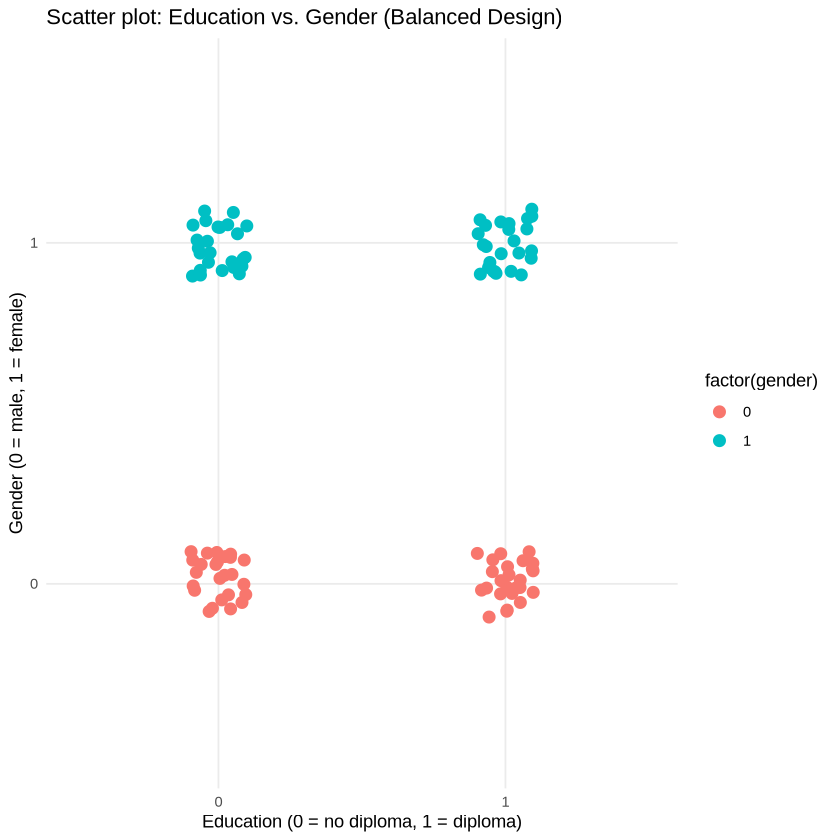
\includegraphics[width=0.5\textwidth]{example_correlation.png}
                \caption{visual representation of uncorrelated variables
                }
                \label{fig:visual representation of uncorrelated variables}
        \end{figure}
    \end{infobox}
\end{itemize}

\subsubsection{Disambiguation : On the difference between errors and residuals}
\begin{enumerate}
    \item Errors ($u_i$) : 
    \begin{itemize}
        \item Definition : The true, unobservable difference between the actual value and the true population regression line (which is the expression for the relation we are trying to estimate through the regression model). It represent inherent randomness in the true population.  
        \subitem - why is there a difference between actual values and the true population parameter : actual (observed) values are sample dependent whereas the true population parameters do not change regardless of which sample we take. 
        \subitem - it cannot be observed directly (we don't know the parameters from the true population !)
        
    \end{itemize}
    \item Residuals ($\hat{u}_i$) : 
    \begin{itemize}
        \item Definition : observable difference between the actual value and the predictor 
        \subitem - formula : $\hat{u}_i=y_i-\hat{y}_i$
        \subitem - it can be estimated from sample data
    \end{itemize}
\end{enumerate}
\begin{linkbox}
\begin{itemize}
    \item Residuals are practical estimates of the unobservable error ! (residuals are proxies)
    \item As sample estimates approach the true parameters, the distribution of residuals approaches the distribution of errors.
\end{itemize}    
\end{linkbox}


\section{Hypothesis testing}

\subsection{General methodology of hypothesis testing}
\begin{enumerate}
    \item Set up the null and alternative hypotheses 
    \item Set the test size
    \item Give the decision rule : 
    \begin{decisionbox}
        \begin{itemize}
          \item \textbf{Two-tailed test}: Reject $H_0$ if $|$test statistic$|$ $>$ critical value
          \item \textbf{One-tailed test (right)}: Reject $H_0$ if test statistic $>$ critical value
          \item \textbf{One-tailed test (left)}: Reject $H_0$ if test statistic $<$ critical value
          \item \textbf{p-value approach}: Reject $H_0$ if p-value $<$ significance level ($\alpha$)
        \end{itemize}
    \end{decisionbox}
    \item Compute the appropriate test statistic and determine its distribution based on : the size of the sample, what you know, what you are trying to test for
    \item Compute the p-value / critical value
    \item Compare the test statistic to the critical value
\end{enumerate}

\subsubsection{Special case : find the estimate of a coefficient in a constrained model}
\begin{enumerate}
    \item take $H_0 : b_1 =b2$ and $b_3+b_1=1$ (alternative hypothesis : no constraints)
    \item rewrite $b_3, b_2$ as a function of $b_1$
    \item replace them in the regression equation and pull together the terms multiplied by $b_1$ (here $x_{1i}+x_{2i}-x_{3i}$
    \item withdraw the extra terms from both sides (here $x_{3i}$)
    \item note X the terms multiplying $b_1$ and Y the expression on the left hand side
    \item get the OLS estimator for a and $b_1$ and express those for $b_2,b_3$ as a function of $\hat{b}_1$
    
\end{enumerate}

\subsection{Important metrics }

\subsubsection{Level of significance (test size)}
\begin{itemize}
    \item Denotes the probability of a type I error (False positive)\footnote{WARNING : it is not possible to minimize both Type I and Type II errors at the same time, there is always a tradeoff}
    \item Definition : 
\begin{equation}
    \alpha = \max_{\theta\in\Omega_0}P_{\theta}(\hat{W}>c)
\end{equation}
\end{itemize}

\subsubsection{Power of a test}
\begin{itemize}
    \item probability of rejecting $H_0$ for any value of $\theta\in\Omega_1$ (True positive)
    \item Definition : 
    \begin{equation}
        \text{power = }P_{\theta\in\Omega_1}(\hat{W}>c_{\alpha})
    \end{equation}
\end{itemize}

\subsubsection{P-value}
\begin{itemize}
    \item simplified : probability that $H_0$ s true (if low enough one can reject $H_0$)
    \subitem - detailed : it tells you the probability of the data given the null hypothesis. In other words, the p-value is a conditional probability that assumes $H_0$ is true before seeing the data.
    \item alternative description : probability of observing a test statistic at least as extreme as the one calculated from your sample data, assuming the null hypothesis is true.
    \item Definition : 
\begin{equation}
    \text{p-value : } \max_{\theta\in\Omega_0}P_{\theta}(\hat{W}>\hat{W}(\omega))
\end{equation}
\end{itemize}

\subsubsection{R-squared and adjusted R-squared}
\begin{itemize}
    \item what does it measures : share of the variation in the dependent variable that is explained by the independent variables considered in the model
    \item property : the regular $R^2$ goes up whenever you add a variable (does not depend on whether the variable in question is orthogonal to existing ones or not)
    \item formulas : with K the number of parameters (excluding the constant)
    \begin{equation}
    \left\{
    \begin{aligned}
            R^2 = \frac{SSE}{SST}\\
            \text{adjusted } R^2 = 1-\frac{SSR/(N-K-1)}{SST/(N-1)}
    \end{aligned}
    \right.
    \end{equation}
\end{itemize}

\subsubsection{Confidence intervals}
\begin{itemize}
    \item formula (for a t-test : $CI(\beta_0)_{1-\alpha} = [\hat{\beta}-t_\alpha\sigma_{\hat{\beta}} < \beta_0 < \hat{\beta}+t_\alpha\sigma_{\hat{\beta}}]$
    \item interpretation : the confidence interval contains the parameter $\beta_0$ with $(1-\alpha)\%$ confidence.
\end{itemize}

\subsection{Useful distributions}

\subsubsection{Chi-square distribution}
\begin{itemize}
    \item condition : $X_1, ..X_n$ i.i.d with $X_i\sim N(\mu,\sigma^2)$
    \item property : 
\begin{equation}
    \sum_{i=1}^n(X_i-\bar{X})^2/\sigma_2 \sim \chi^2(n-1)
\end{equation}
    \item We have N-1 independent elements hence the N-1 degrees of freedom. 
\begin{proofbox}
\begin{itemize}
    \item We have the following constraint : $\bar{X}=\frac{1}{N}\sum_{i=1}^NX_i$
    \item We can rewrite it to express $X_N-\bar{X}$ as a function of $\bar{X}$ and $(X_i)_{i=1}^{N-1}$
\begin{equation}
    (X_N-\bar{X}) = (N-1)\bar{X}-\sum_{i=1}^{N-1}X_i
\end{equation}
\end{itemize}   
\end{proofbox}
    \item properties : independence (if $X\sim \chi_k$ and $Y\sim \chi_n$ with X and Y independent $\Longrightarrow X+Y\sim\chi_{k+n}$)
\end{itemize}

\subsubsection{Student's t-distribution}
\begin{itemize}
    \item Condition : $X_1,..X_n$ i.i.d and Formula : $\sim N(\mu,\sigma^2)$
    \item $\frac{\bar{X}-\mu}{s/\sqrt{n}}\sim t(n-1)$
    \item where s is the estimate for standard deviation 
    \begin{proofbox}
The naive estimator ($\mu$ not known) for the variance is given by:
$$\hat{\sigma}^2 = \frac{1}{N} \sum_{i=1}^{N} (X_i - \bar{X})^2.$$
To check whether $\hat{\sigma}^2$ is unbiased, we compute its expected value:
$$E[\hat{\sigma}^2] = E\left[\frac{1}{N} \sum_{i=1}^{N} (X_i - \bar{X})^2\right].$$
We first note that the sum of squared deviations can be rewritten as:
$$\sum_{i=1}^{N} (X_i - \bar{X})^2 = \sum_{i=1}^{N} (X_i - \mu)^2 - N(\bar{X} - \mu)^2.$$
Taking expectations on both sides:
$$E\left[\sum_{i=1}^{N} (X_i - \bar{X})^2\right] = E\left[\sum_{i=1}^{N} (X_i - \mu)^2\right] - E\left[N(\bar{X} - \mu)^2\right].$$
Since:
$$E\left[\sum_{i=1}^{N} (X_i - \mu)^2\right] = N \sigma^2$$
and
$$E\left[(\bar{X} - \mu)^2\right] = \frac{\sigma^2}{N},$$
We have,
$$E\left[\sum_{i=1}^{N} (X_i - \bar{X})^2\right] = N\sigma^2 - N\left(\frac{\sigma^2}{N}\right) = (N-1)\sigma^2.$$
Thus, the expression for the unbiased estimator is : 
$$s^2 = \frac{1}{N-1}E\left[\sum_{i=1}^{N} (X_i - \bar{X})^2\right]$$
    \end{proofbox}
    \item Properties : symmetric around 0  + lower nb of df implies fatter tails (as nb of dg goes to $\infty$, this distribution converges to the normal distribution)
\end{itemize}

\subsubsection{Fisher distribution}
\begin{itemize}
    \item Condition : $Q_1\sim \chi^2(n_1)$ and $Q_2\sim \chi^2(n_2)$, independent
    \item Formula : $\frac{Q_1/n_1}{Q_2/n_2}\sim F(n_1,n_2)$
\end{itemize}

\subsection{Common tests}

\subsubsection{T-test}
\begin{Tbox}
    \textbf{What is it used for ? :} test hypothesis on individual regression coefficients (works also with single linear restrictions such as "is $\beta_1=\beta_2$")
    \begin{itemize}
        \item set up : $H_0 : \beta_k = c$ with c a constant
        \item test statistic : $\hat{T} = \frac{\hat{b}_k}{\hat{\sigma}_{\hat{b}_k}} \sim t(n-k)$ with k the nb of parameters (including the constant)
        \item decision rule : $|\hat{T}|>t_{1-\alpha/2}(n-k)$\footnote{$t_{1-\alpha}$ decreases in $\alpha$}
    \end{itemize}
\end{Tbox}

\subsubsection{F-tests}
\begin{Fisherbox}
\textbf{What is it used for ? :} (1) test the joint significance\footnote{joint significance of coefficients means that at least one of the coefficients tested is different from 0, H1 : $\exists\beta_k\neq0$} of several coefficients [for instance "is $\beta_1=\beta_2=0$", we have 2 restrictions], (2)  test the relevance of a given model 
\begin{enumerate}
    \item case 1 : testing whether some parameters can be safely removed from the model\footnote{see :  \href{https://www.statisticshowto.com/probability-and-statistics/hypothesis-testing/f-test/}{link with the formula for the F-test} }
    \begin{itemize}
        \item set up : $H_0 :$ there are m linear restrictions (you can safely remove the m parameters of interest and take the restricted model without information loss)
        \item test statistic : $\hat{F}= \frac{(SSR_{r}-SSR_{ur})/m}{SSR_{ur}/(n-k)}\sim F(m,n-k) $ with k the nb of parameters in the unrestricted model (including the constant)
        \item decision rule (reject $H_0$ if): $\hat{F}>F_{1-\alpha}(m, N-K)$
    \end{itemize}
    \item case 2 : test whether all parameters but the constant are equal to zero 
    \begin{itemize}
        \item goal : test whether a model as a whole has any explanatory power beyond just the mean 
        \item set up : $H_0 : \forall i, \beta_i=0$ and $a\neq0$ 
        \item test statistic : $\hat{F}=\frac{R^2_{ur}(n-k)}{(1-R^2_{ur})(k-1)}\sim F(k-1,n-k)$ with k the number of parameters (including the constant)
        \item decision rule : $\hat{F}>F_{1-\alpha(k-1,n-k)}$\footnote{$t_{1-\alpha/2}$ decreases as the number of degrees of freedom rises} or $(k-1)\hat{F} >\chi^2_{1-\alpha}(k-1)$
    \end{itemize}
\end{enumerate}
\end{Fisherbox}

\subsubsection{Wald test}
\begin{Waldbox}
    \textbf{What is it used for ? :} (1) simultaneously test for several parameters using matrices, (2) test for linear combinations of parameters
    \begin{itemize}
        \item set up : $H_0:R\beta_0 =c$, (R is a matrix of dimension MxK)
            \subitem - Example : $g(\beta_0)=0$ with g a continuous function, $g(\beta_0)$ a Mx1 vector and $\beta_0$ a Kx1 vector
        \item test statistic : if $R(\hat{\beta}-\beta_0)\xrightarrow[]{d}N(0,\hat{\sigma}^2R(X'X)^{-1}R')$ then $(R\hat{\beta}-c)\xrightarrow[]{d}N(0,\hat{\sigma}^2R(X'X)^{-1}R')$\footnote{WARNING : if we are using the delta method (as in the example above with g), J depends on $g(\beta_0)$ so we need to take into account the hypothesis we made and evaluate it in 0 when computing the test statistic ! }
        \begin{equation}
        \hat{W}=(R\hat{\beta}-c)'[\hat{\sigma}^2R(X'X)^{-1}R']^{-1}(R\hat{\beta}-c) \xrightarrow[]{d}\chi^2_M 
        \end{equation}
        \item note :  $\hat{W}=\hat{T^2}$ (two side student t test is a wald test)
        \item decision rule : $|\hat{W}|>\chi^2_{1-\alpha}(M)$ with $ \chi^2_{1-\alpha}(M)$ the $1-\alpha$ quantile of the chi-squared distribution with M degrees of freedom.
        \item general property of the Wald test : consistent
    \end{itemize}
\end{Waldbox}

\subsubsection{Consistency of a test}
\begin{itemize}
    \item a test is consistent if : test power = $P_{\theta\in\Omega_1}(\hat{W}>c_{\alpha}) \xrightarrow{n\to\infty}1$
    \item aka : probability of rejecting the null hypothesis when false tends to one
\end{itemize}

\subsection{Other useful results}
\begin{itemize}
    \item standard error : 
    \begin{enumerate}
        \item $SE(\hat{\beta_1}) = \sqrt{V(\hat{\beta)}} = \sqrt{\hat{\sigma}^2(X'X)^{-1}}$ \footnote{we do not divide by $\sqrt{n}$ as the sample size n is already factored into this calculation through the X'X matrix !} 
            \subitem - alternative formula : $SE(\hat{\beta_1})=\sqrt{\frac{SSR}{N-K}(X'X)^{-1}}$
        \item $SE(\bar{x}) = \sqrt{V(\bar{x})} = \sqrt{\frac{\sigma^2}{n}}$ 
    \end{enumerate}
\end{itemize}


\section{Asymptotic theory}
\subsection{Modes of convergence}
\subsubsection{Sure convergence ($\xrightarrow{s}$)}
\begin{itemize}
    \item definition : 
\begin{equation}
    \forall w\in\Omega, \forall\epsilon>0,\exists n_0(w,\epsilon),\forall n\geq n_0\Longrightarrow|X_n(w)-X(w)|<\epsilon
\end{equation}
    \item Pointwise ($\forall w\in\Omega$)
    \item If $n_0$ does not depend on w then we have uniform convergence a.k.a the sequence of functions converges to a limit function in such a way that the speed of convergence does not depend on the point in the domain.
\end{itemize}

\subsubsection{Almost sure convergence $\xrightarrow[]{a.s}$}
\begin{itemize}
    \item Definition :
    \begin{equation}
        P(w:\lim_{n\to\infty)}X_n(w)=X(w))=1
    \end{equation}
    \item Pointwise except for a set of P-probabilities 0 (pointwise convergence is not verified for a negligible set of outcomes)
\end{itemize}

\subsubsection{Convergence in probabilities $\xrightarrow{P}$}
\begin{itemize}
    \item Definition : 
    \begin{equation}
        \forall \epsilon>0, P(w:|X_n(w)-X(w)|>\epsilon) \xrightarrow[n\to\infty]{}0
    \end{equation}
    \item Difference from the limit converges to 0 in probability
    \item Infinitely many n for which $X_n(w) \neq X(w)$
\end{itemize}
\subsubsection{Convergence in quadratic mean ($\xrightarrow{L^2}$)}
\begin{itemize}
    \item Definition  : 
    \begin{equation}
        \lim_{n\to\infty}E(|X_n-X|^2)=0
    \end{equation}
\end{itemize}
\subsubsection{Convergence in distribution ($\xrightarrow[]{d}$)}
\begin{itemize}
    \item Definition : 
    \begin{equation}
        \forall x\in\mathbb{R}, F_n(x)\xrightarrow[]{}F(x)
    \end{equation}
    \item Pointwise
    \item Implies $E(f(X_n)) \xrightarrow{}E(f(X))$ i.i.f f is bounded and continuous ! 
\end{itemize}

\begin{figure}
\begin{center}  
 \begin{tikzpicture}[node distance=4cm, auto]  
   
 % Nodes  
 \node[circle, draw, minimum size=2cm] (as) {a.s};  
 \node[circle, draw, minimum size=2cm, right of=as] (p) {p};  
 \node[circle, draw, minimum size=2cm, above of=p] (L2) {$L^2$};  
 \node[circle, draw, minimum size=2cm, right of=p] (d) {d};  
   
 % Solid arrows  
 \draw[->, thick] (L2) -- (p);  
 \draw[->, thick] (p) -- (d);  
 \draw[->, thick] (as) -- (p);  
   
 % Dotted arrows  
 % Dotted arrows with fixed vertical displacement using shifted anchors  
 % Dotted arrow from p to a.s: shift both endpoints downward by 0.3cm, and attach at west or east sides  
 \draw[->, dashed] ([yshift=-0.3cm]p.west) -- ([yshift=-0.3cm]as.east) node[midway, below] {\shortstack{discrete / \\ subsequence}};  
   
 % Dotted arrow from p to L2: shift both endpoints upward by 0.3cm, attaching on north sides for p and L2  
 \draw[->, dashed] ([xshift=0.3cm]p.north) -- ([xshift=0.3cm]L2.south) node[midway, right] {$X_n$ bounded};  
   
 % Dotted arrow from d to p: shift both endpoints upward by 0.3cm, attaching on west for d and east for p  
 \draw[->, dashed] ([yshift=0.3cm]d.west) -- ([yshift=0.3cm]p.east) node[midway, above] {constant};  
    
   
 \end{tikzpicture}  
 \end{center}
 \caption{Relations between the different modes of convergence}
 \end{figure}


\subsection{Useful definitions and theorems}
\subsubsection{Consistency of an estimator}
\begin{itemize}
    \item \textbf{Definition :} Take $W_n = W_n(X_1,...X_n)$ a sequence of estimators of $\theta$, consistency implies :
\begin{equation}
    \lim_{n\to\infty}P_{\theta}(|W_n-\theta|>\epsilon) = 0 \Longleftrightarrow W_n \xrightarrow[]{P}\theta
\end{equation}
    \item Conditions for existence : 
    \begin{enumerate}
        \item Asymptotically invariant : $\lim_{n\to\infty}V_{\theta}(W_n) = 0$
        \item Asymptotically unbiased : $\lim_{n\to\infty} E_{\theta}(W_n) = \theta \Longleftrightarrow{}\lim_{n\to\infty}E_{\theta}(W_n-\theta)=0$
    \end{enumerate}
\end{itemize}

\begin{consbox}
    \begin{itemize}
        \item univariate case : 
        \begin{enumerate}
            \item condition : i.i.d observations and $cov(u_i,x_i) =0 (\Longleftrightarrow E[u_i|x_i=0])$ and $var(x_i)\neq0$
            \item why ? : 
\begin{equation}
    \hat{b} = \frac{cov_n(y_i,x_i)}{var_n(x_i)} \xrightarrow[]{P} \beta_0 + \frac{cov(u_i,x_i)}{var(x_i)}
\end{equation}
        \end{enumerate}
        \item multivariate case : 
        \begin{enumerate}
            \item condition : $E(x_iu_i)=0(\Longleftrightarrow E[u_i|x_i=0])$ and $E(x_ix_i')$ non singular
            \item why ? : 
\begin{equation}
    \hat{\beta} = \beta_0 + \frac{1}{N}(\sum_{i=1}^Nx_ix_i')^{-1}\frac{1}{N}(\sum_{i=1}^Nx_iu_i) \xrightarrow[]{P} \beta_0 + E(x_ix_i')^{-1}E(x_iu_i)
\end{equation}
        \end{enumerate}
    \end{itemize}
\end{consbox}


\subsubsection{Slutsky theorem (P,d)}
\begin{itemize}
    \item if $X_n\xrightarrow[]{d}X, Y_n\xrightarrow[]{P}c \Longrightarrow X_n+Y_n \xrightarrow[]{d}X+c$ and $X_nY_n\xrightarrow[]{d} cX$\footnote{The weaker form of convergence dominates (here d)}
\end{itemize}
\subsubsection{Continuous mapping theorem (a.s, P, d)}
\begin{itemize}
    \item if $X_n\xrightarrow{}X$ then $g(X_n)\xrightarrow[]{}g(X)$
    \item Condition : g almost continuous (at least)
    \item concrete example : given $E(x_ix_i')$ non singular, $f(A) = A^{-1}$ is continuous on the set of non singular matrix so : $(\frac{1}{N}\sum_{i=1}^Nx_ix_i')^{-1} \xrightarrow[]{P}E(x_ix_i')^{-1}$
\end{itemize}
\subsubsection{Asymptotic equivalence (P $\xrightarrow{}d)$}
\begin{itemize}
    \item if $|X_n-Y_n|\xrightarrow[]{P}0$ and $X_n\xrightarrow[]{d}X$ then $Y_n\xrightarrow[]{d}X$
\end{itemize}
\subsubsection{Law of large numbers (P, a.s)}
\begin{itemize}
    \item Condition : $X_i$ i.i.d + mean is finite (for strong law $E(|X_i|$ must be finite)
    \item Weak/strong law : $\frac{1}{N}\sum_{i=1}^{N}X_i\xrightarrow[]{P/a.s}E(X_i) =\mu$
\end{itemize}

\subsubsection{Central Limit Theorem (d)}
\begin{itemize}
    \item Condition : $X_i$s i.i.d (here, mean is $\mu$ and covariance matrix is $\Sigma$)
    \item Expression : $\sqrt{N}(\bar{X}-\mu) \xrightarrow[]{d}N(0,\Sigma)$
\end{itemize}

\subsection{Methods and results}
\subsubsection{Applying the Delta method(d)}
\begin{itemize}
    \item Take $a_n$ a sequence depending on n, $X_n$ a sequence of rvs and m a constant. 
    \item Property :
\begin{equation}
    a_n(X_n-m) \xrightarrow[]{d}Z \Longrightarrow a_n(f(X_n)-f(m))\xrightarrow[]{d}J(m)Z \text{ with } J(m)=(\frac{\delta f_i(m)}{\delta x_j})_{i,j}
\end{equation}
\end{itemize}
\subsubsection{Useful results}
\begin{itemize}
    \item Sample mean : $\bar{X} = \frac{1}{N}\sum X_i$ and $\bar{X}\xrightarrow[]{P}N(\mu,\theta)$
    \item Sample variance : $V(\bar{X})=\frac{1}{N}\sum V(X_i)$ with $V(X_i)=\sigma^2$ if $X_n$ are i.i.d  
    \item estimated variance of $\hat{\beta}$ : $V(\hat{\beta)}=\sqrt{\tilde{\sigma}^2(X'X)^{-1}}= \sqrt{\frac{1}{N-K}\sum(y_i-x_i'\hat{\beta})^2}$
\end{itemize}
\begin{asymbox}
    \begin{itemize}
        \item OLS(univ.) : $\sqrt{N}(\hat{b}-b_0)\xrightarrow[]{d}N(0,\frac{\sigma_0^2}{Var(x_i)})$
        \item OLS (multiv.) : $\sqrt{N}(\hat{\beta}-\beta_0)\xrightarrow[]{d}N(0,\sigma_0^2E(x_ix_i')^{-1}) = N(0,\sigma_0^2(X'X)^{-1})$
        \item t-test : $t(n)\xrightarrow[]{d}N(0,1)$
        \item F-test : $kF(k,n)\xrightarrow[]{d} \chi^2_k$ (so $k\hat{F}$ is asymptotically equivalent to the wald statistic)
    \end{itemize}
\end{asymbox}

\section{Appendix}

\subsection{A bit of matrix algebra}
\begin{itemize}
    \item For variance computations : 
    \begin{enumerate}
        \item $V(BU) = BV(U)B'$ with B a deterministic matrix and U a vector of random variables
        \item $V(X) = E(XX') - E(X)E(X') = E[(X-EX)(X-EX)']$
        \item using the LIE : $V(X) = E(E((X-EX)^2|X))$
    \end{enumerate}
    \item Playing with transposition : 
    \begin{enumerate}
        \item $E(X') = E(X)'$
        \item $(A+B)'=A'+B'$
        \item $(A^{-1})'=(A')^{-1}$
        \item $(AB)'=B'A'$
        \item For any matrix A : A'A is positive semidefinite ($\Longrightarrow A'A \geq0)$
        \begin{proofbox}
            \textbf{Proof of Positive Semidefiniteness:}\\
    For any vector $x \in \mathbb{R}^m$,with $M=AA^T$
    $$    x^T M x = x^T (A A^T) x = (A^T x)^T (A^T x) = \|A^T x\|^2 \ge 0.    $$
    
    Since the squared norm is always non-negative, $M$ is positive semidefinite.
        \end{proofbox}
    \end{enumerate}
    \item Homoskedacity in matrix form : $V(U|X) = \sigma^2I$ 
\end{itemize}
\subsection{Other useful formulas}
\begin{itemize}
    \item Unbiased variance estimator under homoskedacity : $\hat{\sigma}^2= \frac{\sum_{i=1}^n \hat{u}_i^2}{n-K}$ with K the number of regressors (including the intercept!)
\end{itemize}


\subsection{Table with common distributions}

\begin{table}[H]
\centering
\caption{Probability Distributions -- Part I}
\label{tab:dist_part1}
\renewcommand{\arraystretch}{1.3}
\begin{tabular}{l c c c}
\toprule
\textbf{Distribution} & \textbf{Type} & \textbf{Support} & \textbf{PDF/PMF} \\
\midrule
\makecell{Uniform \\ (Cont.) \\ $\mathcal{U}(a,b)$} & Cont. & $x\in[a,b]$ & $f(x)=\frac{1}{b-a}$ \\
\makecell{Uniform \\ (Disc.) \\ $\mathcal{U}\{a,\dots,b\}$} & Disc. & $x\in\{a,\dots,b\}$ & $P(X=x)=\frac{1}{b-a+1}$\\
\makecell{Normal \\ $N(\mu,\sigma^2)$} & Cont. & $x\in\mathbb{R}$ & $f(x)=\dfrac{1}{\sqrt{2\pi\sigma^2}}\exp\Big(-\dfrac{(x-\mu)^2}{2\sigma^2}\Big)$ \\
\makecell{Exponential \\ $\operatorname{Exp}(\lambda)$} & Cont. & $x\in[0,\infty)$ & $f(x)=\lambda e^{-\lambda x}$ \\
\makecell{Poisson \\ $\operatorname{Pois}(\lambda)$} & Disc. & $x\in\{0,1,2,\dots\}$ & $P(X=x)=\dfrac{\lambda^x e^{-\lambda}}{x!}$ \\
\makecell{Geometric \\ $\operatorname{Geom}(p)$} & Disc. & $x\in\{1,2,3,\dots\}$ & $P(X=x)=(1-p)^{x-1}p$ \\
\makecell{Binomial \\ $\operatorname{Bin}(n,p)$} & Disc. & $x\in\{0,1,\dots,n\}$ & $P(X=x)=\binom{n}{x}p^x(1-p)^{n-x}$ \\
\makecell{Hypergeometric \\ $\operatorname{Hyp}(N,K,n)$} & Disc. & $x\in\{\max(0,n-(N-K)),\dots,\min(n,K)\}$ & $P(X=x)=\dfrac{\binom{K}{x}\binom{N-K}{n-x}}{\binom{N}{n}}$ \\
\makecell{Bernoulli \\ $\operatorname{Bern}(p)$} & Disc. & $x\in\{0,1\}$ & $P(X=x)=p^x(1-p)^{1-x}$ \\
\bottomrule
\end{tabular}
\end{table}

\vspace{1em} % add some vertical space between tables

\begin{table}[H]
\centering
\caption{Probability Distributions -- Part II}
\label{tab:dist_part2}
\renewcommand{\arraystretch}{1.3}
\begin{tabular}{l c c c}
\toprule
\textbf{Distribution} & \textbf{CDF} & \textbf{Expectation} & \textbf{Variance} \\
\midrule
\makecell{Uniform \\ (Cont.) \\ $\mathcal{U}(a,b)$} & $F(x)=\frac{x-a}{b-a}$ & $\frac{a+b}{2}$ & $\frac{(b-a)^2}{12}$ \\
\makecell{Uniform \\ (Disc.) \\ $\mathcal{U}\{a,\dots,b\}$} & $F(x)=\frac{\lfloor x\rfloor - a+1}{b-a+1}$ & $\frac{a+b}{2}$ & $\frac{(b-a+1)^2-1}{12}$ \\
\makecell{Normal \\ $N(\mu,\sigma^2)$} & $F(x)=\Phi\Big(\frac{x-\mu}{\sigma}\Big)$ & $\mu$ & $\sigma^2$ \\
\makecell{Exponential \\ $\operatorname{Exp}(\lambda)$} & $F(x)=1-e^{-\lambda x}$ & $\frac{1}{\lambda}$ & $\frac{1}{\lambda^2}$ \\
\makecell{Poisson \\ $\operatorname{Pois}(\lambda)$} & $F(x)=\sum_{k=0}^{\lfloor x\rfloor}\frac{\lambda^k e^{-\lambda}}{k!}$ & $\lambda$ & $\lambda$ \\
\makecell{Geometric \\ $\operatorname{Geom}(p)$} & $F(x)=1-(1-p)^{\lfloor x\rfloor}$ & $\frac{1}{p}$ & $\frac{1-p}{p^2}$ \\
\makecell{Binomial \\ $\operatorname{Bin}(n,p)$} & $F(x)=\sum_{k=0}^{\lfloor x\rfloor}\binom{n}{k}p^k(1-p)^{n-k}$ & $np$ & $np(1-p)$ \\
\makecell{Hypergeometric \\ $\operatorname{Hyp}(N,K,n)$} & $F(x)=\sum_{k=\max(0,n-(N-K))}^{\lfloor x\rfloor}\dfrac{\binom{K}{k}\binom{N-K}{n-k}}{\binom{N}{n}}$ & $\frac{nK}{N}$ & $\frac{nK(N-K)(N-n)}{N^2(N-1)}$ \\
\makecell{Bernoulli \\ $\operatorname{Bern}(p)$} & 
\makecell{$F(x)=\begin{cases} 0, & x<0 \\[5pt] 1-p, & 0\le x<1 \\[5pt] 1, & x\ge 1 \end{cases}$} & $p$ & $p(1-p)$ \\
\bottomrule
\end{tabular}
\end{table}

\subsection{Table of common estimators}


%-----------------------------------------------------------
% Part I: Known/Assumed Information, Parameter/Hypothesis, and Estimator/Test Statistic
%-----------------------------------------------------------
\begin{table}[H]
\centering
\caption{Summary of Statistical Estimators and Their Distributions: Part I}
\label{tab:estimators_part1}
\renewcommand{\arraystretch}{1.3}
\begin{tabular}{@{}p{5cm} p{4cm} p{6cm}@{}}
\toprule
\textbf{Known/Assumed Information} & \textbf{Parameter/Hypothesis} & \textbf{Test Statistic} \\
\midrule
$\sigma^2$ known  & Mean $\mu$ & 
$Z = \dfrac{\bar{x} - \mu}{\sigma/\sqrt{n}}$ \\[5pt]
\midrule
$\mu$ known  & Variance $\sigma^2$ & 
$\chi^2 = \dfrac{n\sum (x_i-\mu)^2}{\sigma^2}$ 
(or, for a sample, $\chi^2 = \dfrac{(n-1)s^2}{\sigma^2}$) \\[10pt]
\midrule
Neither known  & Mean $\mu$ &
$t = \dfrac{\bar{x} - \mu}{s/\sqrt{n}}$ \\[5pt]
\midrule
Neither known  & Variance $\sigma^2$ &
$\chi^2 = \dfrac{(n-1)s^2}{\sigma^2}$ \\[5pt]
\midrule
$\sigma^2$ known  & Proportion $p$ &
$Z = \dfrac{\hat{p} - p}{\sqrt{\dfrac{p(1-p)}{n}}}$ \\[5pt]
\midrule
Neither known  & Difference in Means $(\mu_1-\mu_2)$ &
$t = \dfrac{(\bar{x}_1-\bar{x}_2) - (\mu_1-\mu_2)}{s_p\sqrt{\frac{1}{n_1}+\frac{1}{n_2}}}$ \\[5pt]
\midrule
Multivariate case; Covariance matrix known  & Vector of Means $\mu$ &
$T^2 = n(\bar{x}-\mu)'\Sigma^{-1}(\bar{x}-\mu)$ \\[5pt]
\midrule
Regression (parameters unknown)  & Individual Coefficient $\beta$ &
$t = \dfrac{\hat{\beta} - \beta}{SE(\hat{\beta})}$ \\[5pt]
\midrule
Regression (overall test)  & Overall Model Significance \newline (e.g. $H_0: \beta_1=\beta_2=\cdots=0$) &
$F = \dfrac{MS_\text{regression}}{MS_\text{error}}$ \\
\bottomrule
\end{tabular}
\end{table}

\vspace{1em}

%-----------------------------------------------------------
% Part II: Known/Assumed Information and Distribution
%-----------------------------------------------------------
\begin{table}[H]
\centering
\caption{Summary of Statistical Estimators and Their Distributions: Part II}
\label{tab:estimators_part2}
\renewcommand{\arraystretch}{1.3}
\begin{tabular}{@{}p{5cm} p{3.5cm}@{}}
\toprule
\textbf{Known/Assumed Information} & \textbf{Distribution} \\
\midrule
$\sigma^2$ known  & $N(0, 1)$ \\[5pt]
\midrule
$\mu$ known & $\chi^2_{(n)}$ or $\chi^2_{(n-1)}$ \\[5pt]
\midrule
Neither known  & $t_{(n-1)}$ \\[5pt]
\midrule
Neither known  & $\chi^2_{(n-1)}$ \\[5pt]
\midrule
$\sigma^2$ known  & $N(0, 1)$ \\[5pt]
\midrule
Neither known & $t_{(n_1+n_2-2)}$ \\[5pt]
\midrule
Multivariate case; Covariance matrix known & $\chi^2_{(p)}$ \\[5pt]
\midrule
Regression (parameters unknown) & $t_{(n-k)}$ \\[5pt]
\midrule
Regression (overall test) & $F_{(k-1, n-k)}$ \\
\bottomrule
\end{tabular}
\end{table}

\subsection{Hypothesis Testing Reference Tables}

\begin{table}[H]
\centering
\begin{tabular}{|p{3cm}|p{2.5cm}|p{4cm}|p{2.5cm}|p{4cm}|}
\hline
\textbf{Test Type} & \textbf{Null Hypothesis} & \textbf{Test Statistic} & \textbf{Distribution} & \textbf{When to Use} \\
\hline
One-sample z-test & $\mu = \mu_0$ & $W = \frac{\bar{x} - \mu_0}{\sigma/\sqrt{n}}$ & Standard Normal (Z) & Testing a population mean with known variance \\
\hline
One-sample t-test & $\mu = \mu_0$ & $\hat{T} = \frac{\bar{x} - \mu_0}{s/\sqrt{n}}$ & t-distribution with $(n-1)$ df & Testing a population mean with unknown variance \\
\hline
Two-sample t-test (independent) & $\mu_1 = \mu_2$ & $t = \frac{\bar{x}_1 - \bar{x}_2}{\sqrt{\frac{s_1^2}{n_1} + \frac{s_2^2}{n_2}}}$ & t-distribution with df calculated using Welch's approximation & Comparing means of two independent groups \\
\hline
One-proportion z-test & $p = p_0$ & $z = \frac{\hat{p} - p_0}{\sqrt{\frac{p_0(1-p_0)}{n}}}$ & Standard Normal (Z) & Testing a population proportion \\
\hline
Two-proportion z-test & $p_1 = p_2$ & $z = \frac{\hat{p}_1 - \hat{p}_2}{\sqrt{\hat{p}(1-\hat{p})(\frac{1}{n_1} + \frac{1}{n_2})}}$ & Standard Normal (Z) & Comparing proportions from two populations \\
\hline
F-test (variance ratio) & $\sigma_1^2 = \sigma_2^2$ & $\hat{F} = \frac{s_1^2}{s_2^2}$ & F-distribution with $(n_1-1, n_2-1)$ df & Comparing variances of two populations \\
\hline
\end{tabular}
\caption{Common Hypothesis Tests}
\end{table}

\begin{table}[H]
\centering
\begin{tabular}{|p{3.5cm}|p{3cm}|p{4cm}|p{2.5cm}|p{3.5cm}|}
\hline
\textbf{Test Type} & \textbf{Null Hypothesis} & \textbf{Test Statistic} & \textbf{Distribution} & \textbf{When to Use} \\
\hline
t-test for regression coefficient & $\beta = c$ (a constant) & $t = \frac{\hat{\beta}-c}{SE(\hat{\beta})}=\frac{\hat{b_k}}{\hat{\sigma_{\hat{b_k}}}}$ \tablefootnote{see : note about error terms page 2 for more details on the SE} & t-distribution with $(n-k)$ df & Testing significance of individual regression coefficients \\
\hline
F-test for relevance of overall regression model & All $\beta = 0$ (excluding constant) & $\hat{F}=\frac{(TSS-RSS)(n-k)}{(1-RSS)(k-1)}$\tablefootnote{\href{https://www.stat.berkeley.edu/~rabbee/s154/ISLR_First_Printing.pdf}{see : page 90 in this book}} & F-distribution with $(k-1, n-k)$ df & Testing if any predictors are significant \\
\hline
F-Test (restricted vs unrestricted model) & $\beta_1$ and $\beta_2$ are equal to 0  & $\hat{F}= \frac{(R_{ur}^2-R^2_r)/q}{(1-R^2_{ur})/(n-k)}$\tablefootnote{q is the number of restrictions, k is the number of predictors in the unrestricted model(including constant)} & F-distribution with $(q,n-k)$ df & Testing for joint significance of two variables \\
\hline
\end{tabular}
\caption{Regression-Based Tests}
\end{table}

 \section{Quick Stata Guide}  
   
 \begin{itemize}[leftmargin=*,itemsep=8pt]  
     \item \textcolor{statablue}{\textbf{tabstat}} \texttt{X Z, statistics(mean)}   
       
     Returns summary statistics for variables X and Z, computing and displaying the mean for each variable.  
       
     \begin{tcolorbox}[colback=lightgray!50,colframe=lightgray!20,boxrule=0.5pt]  
     \texttt{tabstat income education, statistics(mean)}  
     \end{tcolorbox}  
   
     \item \textcolor{statablue}{\textbf{reg}} \texttt{Y X}   
       
     Regresses Y on X (runs a linear regression).  
       
     \begin{tcolorbox}[colback=lightgray!50,colframe=lightgray!20,boxrule=0.5pt]  
     \texttt{reg wage education}  
     \end{tcolorbox}  

    \item \textcolor{statablue}{\textbf{corr}} \texttt{Y X}   
       
     Computes the correlation between variable Y and X.  
       
     \begin{tcolorbox}[colback=lightgray!50,colframe=lightgray!20,boxrule=0.5pt]  
     \texttt{corr wage education}  
     \end{tcolorbox}  
   
     \item \textcolor{statablue}{\textbf{predict}} \texttt{predicted\_values}   
       
     Computes and stores the fitted values in a new variable named \textit{predicted\_values}.  
       
     \begin{itemize}  
         \item For residuals: \textcolor{statablue}{\textbf{predict}} \texttt{new\_variable\_name, res}  
           
         Gets the residuals and stores them in a new variable.  
           
         \begin{tcolorbox}[colback=lightgray!50,colframe=lightgray!20,boxrule=0.5pt]  
         \texttt{predict wage\_hat}\\  
         \texttt{predict residuals, res}  
         \end{tcolorbox}  
     \end{itemize}  
   
     \item \textcolor{statablue}{\textbf{egen}} \texttt{name\_of\_variable = sum(X)}   
       
     Computes the sum of all values in variable X and stores it in a new variable.  
       
     \begin{itemize}  
         \item Why use \textbf{egen} instead of \textbf{generate}:  
           \begin{itemize}  
             \item Enables more advanced operations (min, max, percentiles, etc.)  
             \item Can operate across columns or rows (row means, etc.)  
             \item Handles group-level calculations efficiently  
           \end{itemize}  
             
         \begin{tcolorbox}[colback=lightgray!50,colframe=lightgray!20,boxrule=0.5pt]  
         \texttt{egen total\_income = sum(income)}\\  
         \texttt{egen avg\_by\_group = mean(score), by(group)}  
         \end{tcolorbox}  
     \end{itemize}  
   
     \item \textcolor{statablue}{\textbf{ereturn list}}   
       
     When used after a regression, displays:  
     \begin{enumerate}[label=\arabic*., leftmargin=*]  
         \item Vector of estimated coefficients  
         \item Covariance matrix of estimators  
         \item Log likelihood (when applicable)  
         \item Model statistics: $R^2$ (including adjusted), F-statistic, number of observations, etc.  
     \end{enumerate}  
   
     \item \textcolor{statablue}{\textbf{display}} \texttt{e(r2)}   
       
     Displays the $R^2$ from the most recently estimated regression model.  
       
     \begin{itemize}  
         \item To retrieve estimates from a specific model:  
           
         \begin{tcolorbox}[colback=lightgray!50,colframe=lightgray!20,boxrule=0.5pt]  
         \texttt{* Run model}\\  
         \texttt{reg prate mrate}\\  
         \texttt{* Store results}\\  
         \texttt{estimates store model1}\\  
         \texttt{* Retrieve stored results}\\  
         \texttt{estimates restore model1}\\  
         \texttt{* Display result}\\  
         \texttt{display e(r2)}  
         \end{tcolorbox}  
     \end{itemize}  
   
     \item \textcolor{statablue}{\textbf{gen}} \texttt{mrate\_r = round(mrate, 0.1)}   
       
     Creates a new variable with the values of mrate rounded to the nearest 0.1.  
       
     \begin{tcolorbox}[colback=lightgray!50,colframe=lightgray!20,boxrule=0.5pt]  
     \texttt{gen age\_rounded = round(age, 5)}  
     \end{tcolorbox}  
   
     \item \textcolor{statablue}{\textbf{bysort}} \texttt{mrate\_r:} \textcolor{statablue}{\textbf{egen}} \texttt{prate\_mean = mean(prate)}   
       
     Sorts data by mrate\_r in ascending order, creates groups based on unique values, then calculates the average of prate for each group.  
       
     \begin{tcolorbox}[colback=lightgray!50,colframe=lightgray!20,boxrule=0.5pt]  
     \texttt{bysort education: egen avg\_wage = mean(wage)}  
     \end{tcolorbox}  
   
     \item \textcolor{statablue}{\textbf{twoway}} \texttt{(}\textcolor{statablue}{\textbf{scatter}} \texttt{prate\_mean mrate\_r) (}\textcolor{statablue}{\textbf{line}} \texttt{pred mrate), name(scatterplot\_bins\_fitted,} \textcolor{statablue}{\textbf{replace}}\texttt{)}   
       
     Creates a 2D graph combining multiple plot types. This example overlays:  
     \begin{itemize}  
       \item A scatter plot of prate\_mean against mrate\_r (binned averages)  
       \item A line plot of pred against mrate (fitted values)  
     \end{itemize}  
       
     \begin{tcolorbox}[colback=lightgray!50,colframe=lightgray!20,boxrule=0.5pt]  
     \texttt{twoway (scatter wage education) (line wage\_hat education), \\  
     title("Wage by Education") name(wage\_plot, replace)}  
     \end{tcolorbox}  
      \item \textcolor{statablue}{\textbf{label define}} \texttt{lbl 1 "no degree" 2 "low degree" 3 "high degree"}    
 Creates a new label set named \texttt{lbl} and assigns a specific label to each option (3 in this example).  
   
 \begin{itemize}[leftmargin=*, itemsep=4pt]  
   \item To assign the defined labels to a variable, use:    
   \textcolor{statablue}{\textbf{label values}} \texttt{variable\_without\_labels lbl}  
 \end{itemize}  
   
 \item Using the \textcolor{statablue}{\textbf{if}} function:    
 \textcolor{statablue}{\textbf{scatter}} \texttt{salfr adfe if adfe != 0 \& adfe != 99, name(scatterplot\_wage\_adfe1, replace)}    
 \begin{itemize}[leftmargin=*, itemsep=4pt]  
   \item Enables filtering of observations by excluding specific values (here, 0 and 99) for \texttt{adfe}.  
   \item Can be used in plots, regressions, and other commands to restrict the analysis to a subset of the data.  
 \end{itemize}  
   
 \item \textcolor{statablue}{\textbf{\_pctile}} \texttt{lw, p(.5,99.5)}    
 Calculates the 0.5th and 99.5th percentiles for the variable \texttt{lw} and stores them \textbf{temporarily} in Stata's return memory.  
   
 \item \textcolor{statablue}{\textbf{return list}} versus \textcolor{statablue}{\textbf{global}}    
 \texttt{global p0050 = r(r1)}    
 \begin{itemize}[leftmargin=*, itemsep=4pt]  
   \item \textbf{Using \texttt{return list}:}    
     Displays all returned results from the most recent command (including various computed values, not just the percentiles).  
   \item \textbf{Using the \texttt{global} approach:}    
     \texttt{global p0050 = r(r1)} stores the desired value in Stata's global memory, making it available across all commands and do-files during the session.  
     \begin{itemize}[leftmargin=*, itemsep=3pt]  
       \item \textbf{Example:}    
       \begin{tcolorbox}[colback=lightgray!50, colframe=lightgray!20, boxrule=0.5pt]  
       \texttt{global p0050 = r(r1)}  
       \end{tcolorbox}  
       This command takes the value returned in \texttt{r(r1)} (e.g., the 0.5th percentile from a previous \texttt{\_pctile} command) and stores it in a global macro named \texttt{p0050}.  
     \end{itemize}  
 \end{itemize}  
\end{itemize}

\end{document}
